{
\setlength{\parindent}{2em}
\chapter{State of the Art}\label{cha:state-of-the-art}
Saving the state of a running application to a file has been a very well-known challenge in the world of computer science, one that has its roots back to when the computers became powerful enough to run complicated programs. With the rise of local networks and the Ethernet protocol in the 1970s, an increasing amount of processing units could be linked together through a local network in order to improve the execution speed of difficult computation \cite{book:andrews}. This gave rise to the field of distributed computing, where scalability, parallelization of algorithms and efficient inter-node communication are among the very active topics of research.

Of course, the more complicated a system is, the more failure-prone it becomes. This is why it's imperative for designers of parallel algorithms to be careful when programming their application. It has to be made in such a way that it stays tolerant to eventual faults in the computing nodes of the network. For instance, one can think of the algorithms involved in numerical weather prediction software, that theoretically never finish as long as updated data is fed into the system. It is important for the forecasting industry not to loose any of the results that were previously solved if an unfortunate event occurs. \textit{Fault-tolerant computing} is the research field that finds solutions to this problem in multiple ways. In the context of distributed computing, one of the ways to mitigate the problem is to use a checkpoint and restart mechanism.

This technique allows the program to save itself while it's running, and to restart at a previous checkpoint. A "save" can take many forms, and its content is ultimately decided by the developers of the program. Before a final design is produced, some questions need to be answered:
\begin{enumerate}
	\item \textbf{What needs to be saved?} There needs to be a clear understanding of the program and how it works. Is saving only the intermediate result of a computation considered a sufficient condition to be able to restore the program back to where it was? Is saving the entire state of the operating system required? Of the entire computer? 
	\item \textbf{In which format should the data be saved?} This can be binary data, numerical data, text, etc. This is again highly dependent on the application. A suitable file format has to be used depending on the data to store.
	\item \textbf{How is the data saved?} How can a checkpoint take form? This depends on the content. Most of the time, this will be a file written to non-volatile memory. Again, the file format has a role to play.
	\item \textbf{How often is saving necessary?} A checkpoint can take a lot of space, and that amount usually grows linearly with the number of execution threads. In huge systems, this is not a trivial question. In addition, not only does a checkpoint take up hard disk space, it also induces an overhead in the execution of the program. Depending on the desired granularity, saving the relevant data can take a significant amount of time. This is represented by $O_F$ in \autoref{fig:chkpt-scheme}. This factor is important, especially in big distributed systems where computing time is expensive. As an example, the Titan supercomputer in the United States racks up \$9 million USD in electricity bills yearly \cite{online:henn}.
	\item \textbf{How long does it take to restart?} Saving at checkpoints takes time, but so does recovery. \autoref{fig:chkpt-scheme} shows this with $R_F$. Another point to consider is how often the system needs to restart back. In the end, restarting to a past state must be as straightforward as possible.
\end{enumerate}
\begin{figure}[H]
	\centering
	\includesvg[width=0.9\linewidth]{svg/chkpt-copy}
	\caption{Checkpoint/restart as a stochastic renewal reward process.\cite{misc:chkpt-scheme}}
	\label{fig:chkpt-scheme}
\end{figure}

\subsection*{Checkpointing Schemes}
There are different checkpointing schemes that are adapted to different needs. On one hand, it is possible to checkpoint the application at predetermined intervals $\Delta t$ (i.e every minute). This is useful when applicable, because it puts an upper bound on the amount of data/time loss in a worst case scenario. However, this mitigation method is not always possible for every type of computation. 

The second approach is to do it sporadically. This can be used when it's impossible to predict the amount of time required for a given computation. Unfortunately, it also means that the user doesn't know exactly when checkpoints will occur nor can she/he upper-bound the maximum amount of data/time loss.

\subsection*{Applicability to BBPSim}
Why exactly can these concepts be useful in the case of a simulator like BBPSim? The checkpoint and restart technique is not only applicable to the distributed computing, it can be adapted to fit the needs of multiple kinds of programs. At the very least, some of the concepts can serve as inspiration to design a save \& restore feature. In the following sections, some existing \textit{snapshotting} solutions in released software will be investigated. Using available source code, it will be possible to see that a checkpoint/restart feature can be implemented at different levels. Subsequently, the potential applicability of each implementation will be evaluated. In the end, the analysis will extract a set of working ideas to gather inspiration for the save \& restore in BBPSim.

%---state of the art analysis
\section{VirtualBox}\label{sec:virtualbox}
This open-source software project backed by Oracle is well-known in the virtualization industry. It is a hypervisor, a type of program defined by Red Hat as a
\begin{shadedquotation}
	[...] software that creates and runs [one or more] \gls{VM}. A hypervisor, sometimes called a \gls{VMM}, isolates the hypervisor operating system and resources from the virtual machines and enables the creation and management of those VMs.\cite{online:redhat}
\end{shadedquotation}
Indeed, VirtualBox acts as a mediator between a guest OS (the \textit{virtualized} OS) and a host OS. It is labeled as a Type-2 hypervisor, meaning that it is actually a software layer that separates both operating system, as \autoref{fig:layerhyper} shows. VirtualBox is in charge of exposing computer utilities to the guest operating system, like CPU time, RAM allocation, driver and graphics card access, etc. Like most of its counterparts, the hypervisor also offers to the user the possibility of manually (\textbf{sporadically}) \textit{snapshotting} a virtual machine's current state in order to allow a future restore to exactly this state : the state of the drivers, running process scheduling information, even the graphical interface. The feature outputs a sizable file as a result.

\begin{wrapfigure}{r}{0.45\textwidth}
	\centering \scriptsize
	\vspace{-12pt}
	\includesvg[width=0.37\textwidth]{svg/hypervisor}
	\caption{Abstraction layers for a type-2 hypervisor.}
	\label{fig:layerhyper}
	\vspace{-24pt}
\end{wrapfigure}
This application being open-source, it's possible to dive deeper and investigate the code ourselves \cite{online:vboxcode}. We are mostly interested here at how VirtualBox handles the saving of guest OS processes and memory, since BBPSim doesn't have a graphical interface nor uses the typical PC peripherals like USB or the audio output.

From the root of the code repository, we can find the \pathmono{src/VBox/Main/src-server/SnapshotImpl.cpp} file that contains interesting \Cpp classes and routines. We can see that \cppsym{SessionMachine::i_takeSnapshotHandler} is the method responsible for the snapshot feature. The feature does many things, but four snapshot aspects stand out by how they approached their design to make the saving problem possible.

\subsection*{Snapshotting process}

VirtualBox needs an efficient strategy to save the general state of the virtual machine. Precisely, it is VBox's Saved State Manager's (SSM) responsibility to implement the facilities for saving and restoring a VM state in a structural manner.

During initialization of a given virtual machine (i.e right before the guest OS starts its boot sequence), the SSM registers the different virtual components that are available to the virtualized operating system. When time comes for the user to hit the \inlinegraphics{art/take-snap.png} button while the VM is running, the Saved State Manager goes through its list of registered components. The components then save their internal state themselves using the API the SSM provides, and the SSM takes care of encoding the data. As a result, what is called a "stream" in the project is produced from the agglomeration of the saved data. This is a powerful way of dealing with this problem and has many advantages :
\begin{enumerate}
	\item Encapsulation is kept since each component takes care of saving itself. This is good for software maintenance.
	\item Adding a new component to include in a save only requires it to register itself at initialization. The SSM doesn't need to be aware of the capabilities said component provides.
	\item The time to save a machine's state grows linearly with the number of components, since they are completely decoupled from each other.
\end{enumerate}

\hfill\textit{Relevant file }: \pathmono{src/VBox/VMM/VMMR3/SSM.cpp}.

\subsection*{Non-volatile Memory Snapshot}

From a hard disk point of view, the hypervisor takes an interesting \textit{diff}-based approach. This means that from the time a snapshot is created, VirtualBox associates it with a list $L$ of changes in which all $n$  subsequent hard disk write operations $w$ are added. When the user wants to comeback to a certain snapshot taken at time $t_0$, the \gls{VMM} then takes the current state of the disk ($\text{HDD}_{tn}$) and traverses $L$ in the reverse order while applying the inverse operation.
\[
\text{HDD}_{t0} = \text{HDD}_{tn} + \sum_{i=n}^{0}w_i^{-1}
\]
This effectively undos all previous operations. Using this technique means that \ul{VirtualBox snapshots are dynamic objects} that grow linearly with the subsequent usage of their affiliated VM.

\hfill\textit{Relevant file }: \pathmono{src/VBox/VMM/VMMR3/SSM.cpp}.

\subsection*{CPU State Snapshot}

As for the saving of the CPU state itself, the CPU Monitor (CM) is responsible for keeping track of all the CPU and \gls{FPU} registers while the virtual machine is running. In practice, the exact identity of all those registers depends on the architecture of the host hardware (assumed to be x86) and the host OS. For instance, a 32-bit OS would be using the "extended" (\textit{E}-prefixed) registers, like in \autoref{fig:x86-regs}. 
\begin{figure}[H]
	\centering
	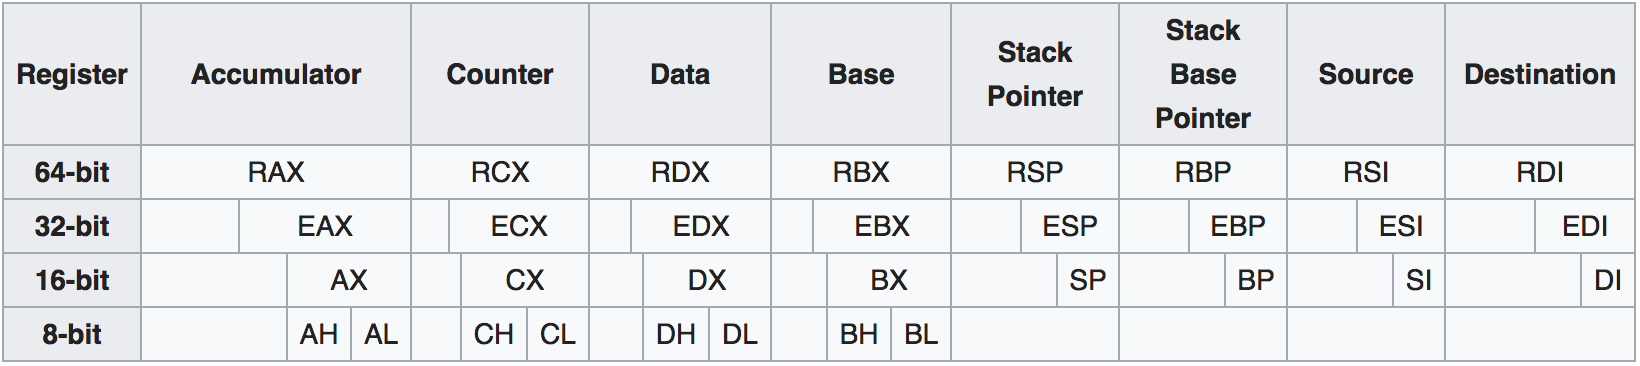
\includegraphics[width=.85\linewidth,keepaspectratio]{art/x86-regs.png}
	\caption{Usage of basic registers ordered by word size of the operating system on the x86 architecture.}
	\label{fig:x86-regs}
\end{figure}
The state (i.e value) of all the relevant CPU registers at a time $t$ is called a \textbf{context}. In VirtualBox, the CM keeps local copies of three of these contexts : a guest OS context, a special hypervisor context for the VMM and a raw context (a normal host OS context). When making a snapshot of the VM, the CPU Monitor actually saves the first two in order to subsequently put back the CPU exactly like it was at time $t$. Beside the saving aspect, holding three different contexts also allows VirtualBox to quickly switch between the guest and host "worlds" without the user noticing. This is very much necessary, because the whole point of the hypervisor is to make two different operating system coexist at the same time.

\hfill\textit{Relevant file }: \pathmono{src/VBox/VMM/VMMR3/CM.cpp}.

\subsection*{RAM Snapshot}

Another extremely important aspect of the state save is the dynamic memory aspect. How can VirtualBox completely separate the guest OS from the host without the guest noticing? This is done through the Page Manager (PM), a manager also taken into account by the Saved State Manager at snapshot time. 

\begin{wrapfigure}{l}{0.45\textwidth}
	\centering \scriptsize
	\vspace{-12pt}
	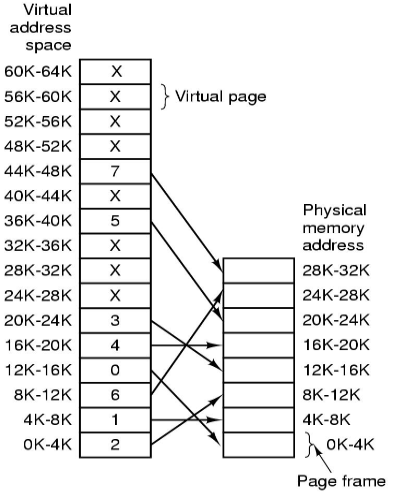
\includegraphics[width=0.40\textwidth,keepaspectratio]{art/mem-paging.png}
	\caption{Linux Mapping of Pages to Page Frames \cite{misc:mem-paging}}
	\label{fig:mem-paging}
	\vspace{-12pt}
\end{wrapfigure}
To better understand the Page Manager's job, we can look at a very similar concept : the memory paging technique used by the Linux operating system. As shown in \autoref{fig:mem-paging}, the way Linux abstracts the hardware from a running program is by offering said program an entire virtual address space as a sandbox. 

This virtual space is divided into fixed-length memory blocks (usually 4kB) called virtual pages that have a one-to-one correspondence to a random block of the same size in physical memory (page frame). Linux abstracts that correspondence with the help of a \gls{MMU} implemented in hardware, which translates virtual addresses into physical ones.

In the same way that Linux controls VirtualBox's physical memory accesses, the Page Manager controls the guest OS memory accesses. It enables the management of pages of memory allocated by the guest and adds one more level of memory indirection. For example, a program running on the guest OS will be executing operations on guest memory, but VirtualBox actually redirects them to operate directly on the physical address space offered by the host OS. This can be done with the help of two powerful concepts:
\begin{enumerate}
	\item \textbf{Binary translation}. This allows a software-assisted hypervisor like VirtualBox to "trap and virtualize the execution of sensitive, non-virtualizable instructions sets"\cite{online:virtualization}, like memory operations.
	\item \textbf{\gls{SLAT}}. Commonly known as \textbf{nested paging}, it allows a guest operating system to directly access the host's physical memory and thus removing a lot of overhead on memory operations.
\end{enumerate} 

Because the \gls{VMM} can hook to these memory operations in the guest OS, this makes the Page Manager aware of the page frames that belong to the guest OS. As a result, when a snapshot event occurs, the PM goes through its list of guest pages that were in use at that time and saves them. At restore time, this data is copied back someplace else in physical memory, and the translation table is updated accordingly.
 
\hfill\textit{Relevant file }: \pathmono{src/VBox/VMM/VMMR3/PGM.cpp}.
\section{Berkeley Lab Checkpoint/Restart for Linux}\label{sec:blcr}
As mentioned throughout this chapter, the problem of checkpointing a computer program can be solved at multiple levels depending on the needs. The approach that was taken by VirtualBox is very powerful, but it has major drawbacks:
\begin{enumerate}
	\item \textbf{Overhead processing}. The fact that an entire system gets simulated implies that virtualizing an operating system with a type-2 hypervisor like VirtualBox is basically an overhead cost on executing the program. 
	\item \textbf{Granularity}. It checkpoints the whole computer's state instead of one program. This is often too much granularity and can result in very large snapshot files. In the case of \gls{BBPSim}, this would be quite excessive.
	\item \textbf{Dependence on an hypervisor}. If the execution of the program had to happen inside an virtualized operating system, a simulation of the \gls{BBP} would have to rely on the use of an hypervisor. This not desirable, especially for the client.
\end{enumerate}

However, some other techniques can circumvent these limitations by taking by using a differing degree of checkpointing transparency, that is, at which abstraction layer the checkpoint takes place. Walters and Chaudhary define those layers as follows: 
\begin{shadedquotation}
\begin{enumerate}
	\item Hardware-level, additional hardware is incorporated into the processor to
save state.
	\item Kernel-level, the operating system is primarily responsible for checkpointing
running programs.
	\item User-level, a checkpointing library is linked into a program that will be responsible for checkpointing the program independent of the programmer.
	\item Application-level, the checkpointing code is inserted directly into the application by a programmer/preprocessor.
\end{enumerate}
\cite{paper:app-level-chkpt}
\end{shadedquotation}

\gls{BLCR} is one those attempts at creating a user-friendly method for checkpointing a Linux program. It is a program implemented at the Kernel-level, meaning that it is a module add-on to the Linux kernel and should be installed prior to running the user application.

\subsection*{Overview}
\gls{BLCR}'s solution is completely different from the one seen in \autoref{sec:virtualbox}, where checkpointing happens for every program running in the guest OS. It bases itself on the fact that properly controlling a program in a sandbox makes it checkpointable. This sandbox is provided by a kernel daemon, another process that runs in background in the kernel, that knows how to execute a checkpoint on a given program. 
\begin{figure}[htbp]
	\centering \small
	\includesvg[width=0.75\textwidth]{svg/blcr}
	\caption{Abstraction layers for an application sandboxed by BLCR.}
	\label{fig:layerblcr}
\end{figure}

There are several different ways to use \gls{BLCR}. An application-centric use case is shown in \autoref{fig:layerblcr}. To access the required utilities to checkpoint itself, the application code needs to have access to the library at compile-time. At runtime, the library (\pathmono{BLCR.so}) is then dynamically linked to the application code and the kernel-based BLCR process is put in charge of managing the application process' resources via the dynamic library. This management layer is necessary to properly save the application.

Checkpointing a program is done is done via shell commands to the background-running BLCR daemon:
\begin{tcolorbox}
\begin{minted}{bash}
cr_checkpoint --pid <PID>
\end{minted}
\end{tcolorbox}

where \texttt{PID} is the process ID of the checkpointable application. This command can be called programatically by the running application (via a \texttt{system()} call in the code), by another program or even by the user itself. Thus, checkpoints are sporadic in that context.

Once those commands are initiated, the \gls{BLCR} daemon outputs a context file containing the relevant information to restart back the application at this stage. At restore, the user must restart the application from the saved context file with another shell command:
\begin{tcolorbox}
\begin{minted}{bash}
cr_restart <path_to_context>
\end{minted}
\end{tcolorbox}
This fully restores the old application state: virtual address space, registers, thread and process IDs, file descriptors, signals. Basically everything not related to sockets or serial ports is put back the way it was.

%https://crd.lbl.gov/departments/computer-science/class/research/past-projects/BLCR/
%- see also virtualization technology : https://github.com/dmtcp/dmtcp (process-based)


\section{Checkpoint and Restore in User Space}\label{sec:criu}
https://github.com/checkpoint-restore/criu



%https://github.com/dmtcp/dmtcp


%super interesting : http://citeseerx.ist.psu.edu/viewdoc/download?doi=10.1.1.126.8121&rep=rep1&type=pdf
%https://www.usenix.org/legacy/publications/library/proceedings/usenix01/freenix01/full_papers/dieter/dieter_html/paper.html
}